% !TEX root = ../Main.tex

Since the isolation and characterisation of
Graphene in 2004 by Andre Geim and
Konstantin Novoselov, scientists have marvelled over the physical properties and potential
application of Graphene. Being a relatively new material, many aspects and ideas are being
investigated and researched at all times. Graphene yield extreme tensile strength as well as
extreme electric conductivity, yet its structure is fairly simple. Graphene consists solely of
carbon atoms thus making it easy to simulate using specialised software, since carbon atoms are greatly understood in terms of chemical
bonding.
As graphene is a very versatile material the possibilities for research in simulation enviroments are virtually limitless.
Therefore it is basically possible to make experiments limited only by imagination, in order
to discover new properties and possible applications of graphene. This saves resources
before entering the lab, where the simulated reality is tested.

In this rapport we will simulate and analyse the properties of nanomembranes as done in the papir "Visualizing the Motion of Graphene Nanodrums"\cite{Davidovikj2016}, which Figure \cref{Motivation} stems from. It shows how phonos travel through this membranes. However there this article,as many others, focuses on membranes in the micro-scale we will examine if this same phenomenons are found at the nano-scale. To do this we start by considering at ideal system of just one sheet of carbon atoms.
To make a more praticel membrane we will investigate if you can create the same membrane effects if you take a graphene layer and put it on top of a substrate with different sized and shaped holes, to form
form this nanomembrane and this is the that we will be looking at. It is expected possible to create such a nanomembrane at the
size of few tens of nanometers at Nanotech with Block-copolymer lithography or TEM
structuring of a substrate. In a virtual environment, it is possible to simulate phonons
in the graphene atop of these holes in the membrane. The purpose of this project is to
simulate phonons in the nanomembrane and find the optimal conditions for producing
phonons in the terahertz spectrum.

We will employ the software Atomistic ToolKit (ATK) to calculate phonon properties
of membranes as well as performing molecular dynamics of the excited membrane. The
software will enable prompt setup of relevant structures so that more time is free to analysis
and actual simulations.
% \onecolumngrid


% \begin{figure}
%     \centering
%     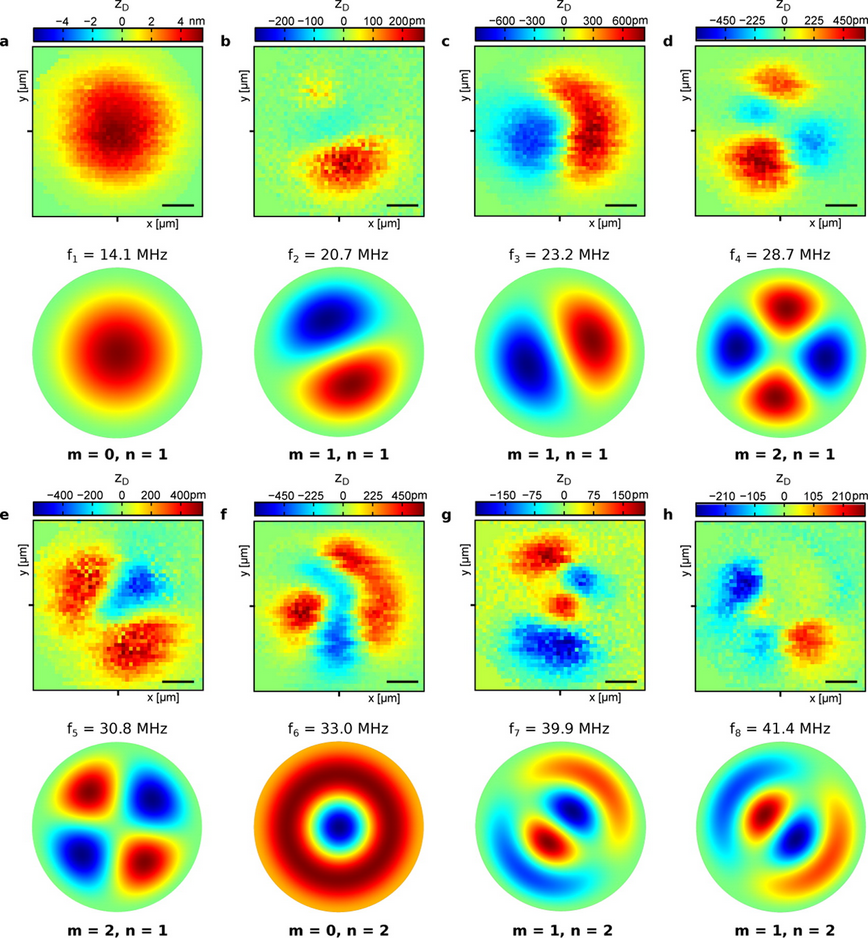
\includegraphics{Figures/NanoDrums.png}
%     \caption{Visualizing resonant motion. (a–h) Top, experimental data; bottom, finite-element calculation. The modes predicted by the calculation are indexed by (m,n). Panels b and c show that the nanodrum hosts a split degenerate (1,1) mode, while also the (2,1) mode is split, as is shown in panels d and e. The displacement profile measured in panel f resembles a (0,2) mode, which is distorted due to an imperfection as discussed in the main text. Panels g and h reveal a degenerate (1,2) mode. Scale bars: 1 μm.\cite{Davidovikj2016}}
%     \label{Motivation}
% \end{figure}
% \twocolumngrid
